\chapter{Masas de los fermiones: quiralidad, acoplamientos de Yukawa y neutrinos de Majorana}

\lectureoverview{Primero reconstruimos el mecanismo de Higgs de los bosones de gauge en una teoría de juguete \(U(1)\) y luego planteamos la pregunta análoga para los fermiones. Una masa de Dirac mezcla campos quirales izquierdos y derechos, pero la interacción débil les asigna cargas distintas y, por tanto, prohíbe una masa desnuda. Un acoplamiento de Yukawa al campo de Higgs respeta la simetría; cuando el campo de Higgs adquiere un valor en el vacío, esa misma interacción se convierte en una masa fermiónica y en un acoplamiento medible de Higgs--fermión. La última parte sigue esta lógica y la aplica a la masa de los neutrinos, a posibles partículas pesadas sin protección, a la cinemática de los rayos cósmicos, a la inercia relativista y a la gravedad.}

El propósito de este repaso inicial no es simplemente repetir la clase anterior. Necesitamos rescatar una idea y expresarla de modo que podamos aplicarla a los fermiones: una masa corresponde a una energía no nula para una excitación de momento nulo. En un campo, momento nulo significa longitud de onda infinita, o un desplazamiento igual en todas partes. Una teoría que solo contiene derivadas no puede detectar un desplazamiento uniforme. Un término sin derivadas sí puede hacerlo.

\section{El mecanismo de los bosones gauge, en pocas palabras}

\subsection{Energía de las derivadas y un vector sin masa}

El campo gauge del modelo es \(A_\mu\), cuya intensidad de campo es
\begin{equation}
  F_{\mu\nu}
  =\partial_\mu A_\nu-\partial_\nu A_\mu .
  \label{eq:l09-field-strength}
\end{equation}
En la pizarra, el término cinético gauge se escribe de forma esquemática como \(F^2\). Con una normalización estándar, es
\begin{equation}
  \mathcal L_{\mathrm{gauge}}
  =-\frac14 F_{\mu\nu}F^{\mu\nu}.
  \label{eq:l09-gauge-kinetic}
\end{equation}

\begin{figure}[htbp]
\centering
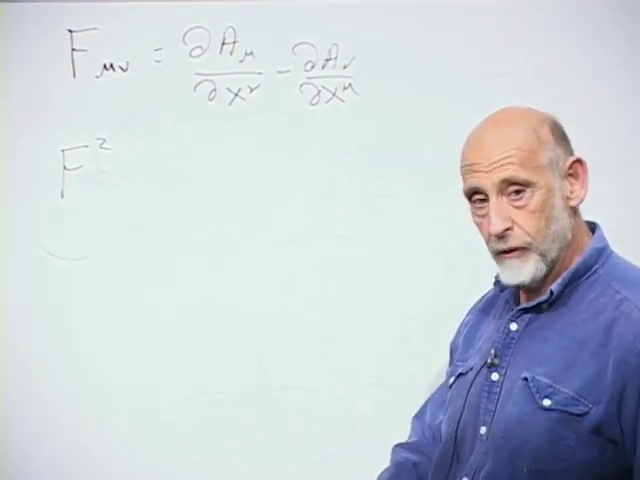
\includegraphics[width=0.72\textwidth]{lecture_09_figure_02.png}
\caption{La definición de la intensidad de campo y la notación abreviada \(F^2\) de la pizarra para la energía de las derivadas del campo gauge.}
\lectureframe{00:02:39}
\label{fig:l09-field-strength-board}
\end{figure}

Cada aparición de \(A_\mu\) en \eqref{eq:l09-gauge-kinetic} está sometida a una derivada. En consecuencia,
\begin{equation}
  A_\mu(x)\longmapsto A_\mu(x)+c_\mu,
  \qquad \partial_\nu c_\mu=0,
\end{equation}
no altera \(F_{\mu\nu}\). Por tanto, un potencial vector homogéneo no cuesta energía de intensidad de campo. En el lenguaje de la clase, el modo de momento nulo no tiene brecha y el bosón gauge no tiene masa.

Este campo \(U(1)\) es un sustituto deliberadamente sencillo. El objetivo físico son los bosones \(W^\pm\) y \(Z\), no el fotón electromagnético. La simetría electromagnética no rota mantiene al fotón sin masa; la simetría electrodébil rota da masa a los bosones gauge débiles.

\subsection{Fijar el módulo del campo de Higgs}

Introduzcamos un escalar complejo cargado y escribámoslo en forma polar:
\begin{equation}
  \phi(x)=\rho(x)e^{i\alpha(x)}.
\end{equation}
El potencial de sombrero mexicano alcanza su mínimo en una circunferencia de radio distinto de cero. Llamemos \(f\) a ese radio; la dirección radial es relativamente rígida. En esta primera aproximación, la fijamos y conservamos solo la fase:
\begin{equation}
  \phi(x)\simeq f e^{i\alpha(x)}.
  \label{eq:l09-frozen-higgs}
\end{equation}

\begin{figure}[htbp]
\centering
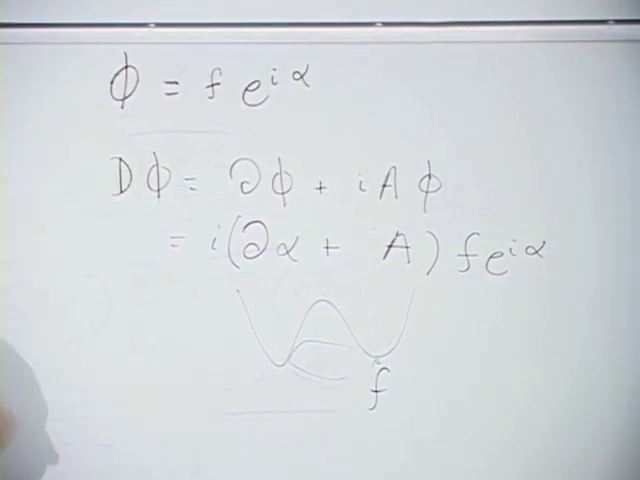
\includegraphics[width=0.72\textwidth]{lecture_09_figure_03.png}
\caption{El módulo fijado del campo de Higgs, su derivada covariante y el pequeño esquema del potencial con simetría rota utilizado en el repaso.}
\lectureframe{00:06:42}
\label{fig:l09-frozen-board}
\end{figure}

Elijamos la convención
\begin{equation}
\begin{aligned}
  D_\mu&=\partial_\mu+igA_\mu,
  \\
  \phi&\longmapsto e^{i\theta}\phi,
  \\
  A_\mu&\longmapsto A_\mu-\frac1g\partial_\mu\theta .
\end{aligned}
  \label{eq:l09-gauge-convention}
\end{equation}
En la clase se omite \(g\); dejarlo explícito permite ver con claridad las dimensiones y la masa que aparece al final. Al actuar sobre el campo con módulo fijado, se obtiene
\begin{align}
  D_\mu\phi
  &=(\partial_\mu+igA_\mu)f e^{i\alpha}
  \notag\\
  &=i\bigl(\partial_\mu\alpha+gA_\mu\bigr)
    f e^{i\alpha}.
  \label{eq:l09-covariant-frozen}
\end{align}
La multiplicación por el conjugado complejo elimina la fase y convierte también \(i\) por \(-i\) en \(+1\):
\begin{equation}
  |D_\mu\phi|^2
  =f^2
   \bigl(\partial_\mu\alpha+gA_\mu\bigr)
   \bigl(\partial^\mu\alpha+gA^\mu\bigr).
  \label{eq:l09-frozen-square}
\end{equation}

\begin{classroomqa}
\audiencequestion{¿Debe llevar un signo menos el cuadrado de la derivada covariante porque la derivada produce un factor de \(i\)?
\lecturetimestamp{00:07:39}}
\lecturerresponse{No. El término cinético es el producto por el conjugado complejo. Un factor aporta \(i\) y el otro \(-i\), de modo que \(i(-i)=1\). La convención de signo para \(D_\mu\) puede invertirse de manera consistente, pero el módulo al cuadrado es positivo en la expresión correspondiente para la energía.}
\end{classroomqa}

La combinación que aparece en \eqref{eq:l09-frozen-square} es por sí misma un campo gauge desplazado. Elijamos \(\theta=-\alpha\), de modo que desaparezca la fase escalar, y definamos
\begin{equation}
  A'_\mu=A_\mu+\frac1g\partial_\mu\alpha .
  \label{eq:l09-unitary-gauge-field}
\end{equation}
Entonces
\begin{equation}
  |D_\mu\phi|^2=g^2f^2 A'_\mu A'^\mu .
  \label{eq:l09-vector-mass-term}
\end{equation}
El nuevo término no contiene derivadas de \(A'_\mu\). Ahora un campo homogéneo almacena energía, así que el modo vectorial de momento nulo tiene una brecha.

\begin{figure}[htbp]
\centering
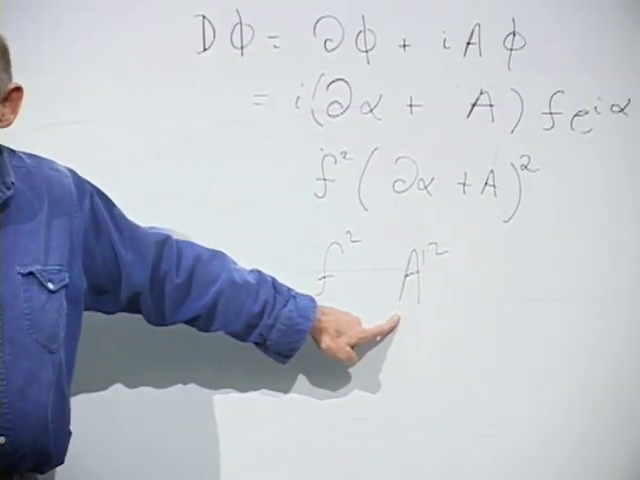
\includegraphics[width=0.72\textwidth]{lecture_09_figure_04.png}
\caption{La pizarra aísla el término \(f^2A^2\) que indica la aparición de una masa para el bosón gauge después de absorber la fase.}
\lectureframe{00:10:31}
\label{fig:l09-vector-mass-board}
\end{figure}

Con la normalización escalar canónica se escribe
\(\phi=(f+h)e^{i\pi/f}/\sqrt2\). Al comparar el término vectorial resultante con
\(\tfrac12m_A^2A_\mu A^\mu\), se obtiene
\begin{equation}
  m_A=gf
  \label{eq:l09-abelian-vector-mass}
\end{equation}
en este modelo abeliano. La clase omite los factores de normalización y resume el resultado diciendo que la masa vectorial viene determinada por \(f\).

La fase no desaparece sin dejar rastro. Antes de introducir el campo gauge, era un bosón de Goldstone sin masa. Una vez introducido, aporta la polarización longitudinal que necesita una partícula vectorial masiva. La fluctuación radial, que por ahora habíamos fijado, permanece como excitación física del Higgs.

\subsection{Por qué un término sin derivadas significa masa}

\begin{classroomqa}
\audiencequestion{¿Por qué se considera que un término \(A'^2\) representa una masa y no simplemente otra interacción?\lecturetimestamp{00:13:10}}
\lecturerresponse{La masa es energía en reposo. Para un campo, una partícula en reposo es el cuanto de un modo de momento nulo y longitud de onda infinita. El término con derivadas no aporta energía a un desplazamiento estático y homogéneo, mientras que \(m_A^2A'^2\) sí lo hace. Esa energía no nula a momento nulo es la brecha de energía en reposo.}
\end{classroomqa}

La clase desarrolla esta idea mediante tres analogías mecánicas.

\begin{itemize}
  \item En un cristal, un desplazamiento que varía lentamente cuesta energía elástica porque los átomos vecinos se desplazan de manera distinta. Una traslación rígida desplaza todos los átomos juntos y no cuesta energía interna. Por eso el fonón acústico no tiene brecha.
  \item En un imán ideal con simetría rotacional, la dirección del espín que varía en el espacio cuesta energía de intercambio, pero girar todos los espines juntos no. La onda de espín asociada, de longitud de onda larga, no tiene brecha.
  \item En un plasma, desplazar el fluido de electrones respecto del fondo positivo produce una separación de cargas y un campo eléctrico restaurador, incluso para un desplazamiento relativo homogéneo. El plasmón resultante tiene una frecuencia distinta de cero cuando el número de onda es nulo.
\end{itemize}

El campo gauge que adquiere masa mediante el mecanismo de Higgs se comporta como el tercer ejemplo: el medio con simetría rota se resiste a lo que, de otro modo, sería un desplazamiento homogéneo sin coste.

\begin{classroomqa}
\audiencequestion{Antes de introducir el campo gauge, ¿la fase \(\alpha\) no oscilaba ya?
\lecturetimestamp{00:18:24}}
\lecturerresponse{Sí. Su energía era proporcional a \(f^2(\partial_\mu\alpha)^2\). Una fase que varía de un lugar a otro tiene energía de gradiente y puede propagarse, pero un cambio uniforme de fase no cuesta energía. Eso es precisamente el modo de Goldstone sin masa.}
\end{classroomqa}

\begin{classroomqa}
\audiencequestion{La derivada incluye una derivada temporal. ¿Mover realmente toda la red o cambiar todo el campo no conlleva energía cinética?
\lecturetimestamp{00:22:18}}
\lecturerresponse{Sí. La comparación es entre configuraciones estáticas o entre configuraciones preparadas con una lentitud arbitraria. Una red que se traslada con velocidad distinta de cero tiene energía cinética. La prueba de la masa pregunta si la configuración conserva energía cuando está en reposo y es uniforme en el espacio.}
\end{classroomqa}

\section{La pista experimental: la interacción débil distingue entre izquierda y derecha}

La clase pasa ahora al electrón, el muón y los quarks. Sus masas también proceden del campo de Higgs, pero el mecanismo tiene otro aspecto porque la masa de un fermión no es un término vectorial cuadrático. Es un acoplamiento entre dos campos quirales.

\subsection{Violación de la paridad en la desintegración beta}

Partamos del hecho empírico de que la interacción débil viola la paridad. La electrodinámica cuántica y la cromodinámica cuántica tratan igual un proceso y su imagen especular. La interacción débil no lo hace. En la desintegración beta del neutrón,
\begin{equation}
  n\longrightarrow p+e^-+\bar\nu_e,
  \label{eq:l09-beta-decay}
\end{equation}
los electrones de alta energía seleccionados por la interacción de corriente cargada tienen helicidad levógira: su espín apunta en sentido opuesto a su momento. Los antineutrinos correspondientes tienen la helicidad opuesta.

Para una partícula ultrarrelativista, definimos la helicidad como
\begin{equation}
  h=\frac{\bm S\cdot\bm p}{|\bm S|\,|\bm p|}.
\end{equation}
El espín paralelo al momento corresponde a \(h=+1\); el espín antiparalelo, a \(h=-1\). La interacción débil se acopla a un campo electrónico quiral izquierdo y a un campo neutrínico quiral izquierdo, pero no de la misma manera a un campo electrónico quiral derecho.\editorialnote{Al principio, la clase emplea «levógiro» y «dextrógiro» en el sentido de la helicidad, porque resulta intuitivo visualizarlo a altas energías. Sin embargo, las cargas gauge actúan sobre la quiralidad, la etiqueta de la representación de Lorentz seleccionada por \(P_L=(1-\gamma^5)/2\) y \(P_R=(1+\gamma^5)/2\). Para una partícula sin masa, la quiralidad y la helicidad coinciden; para una partícula masiva, no.}

Para mostrar el obstáculo sin toda la contabilidad de \(SU(2)_L\times U(1)_Y\), imaginemos un mundo ficticio \(U(1)\) en el que solo \(\psi_L\) lleva la carga pertinente:
\begin{equation}
  \psi_L\longmapsto e^{i\theta}\psi_L,
  \qquad
  \psi_R\longmapsto\psi_R .
  \label{eq:l09-chiral-toy-charge}
\end{equation}
Esto no es electromagnetismo: los electrones reales de quiralidad izquierda y derecha tienen la misma carga eléctrica. Es una caricatura de la interacción débil, en la que las dos quiralidades pertenecen a representaciones electrodébiles distintas.

\begin{classroomqa}
\audiencequestion{¿Se da también en los quarks la misma asimetría izquierda--derecha?
\lecturetimestamp{00:31:50}}
\lecturerresponse{Sí, con los multipletes débiles y las hipercargas correspondientes. Los quarks de quiralidad izquierda, tanto de tipo up como de tipo down, forman dobletes débiles, mientras que los campos de quiralidad derecha son singletes débiles. Por tanto, sus acoplamientos con el Higgs presentan el mismo problema estructural que los del electrón.}
\end{classroomqa}

\section{Una masa de Dirac mezcla los estados de quiralidad izquierda--y derecha}

\subsection{De la ecuación de cuatro componentes a dos ecuaciones de Weyl}

Una función de onda de Dirac tiene cuatro componentes. Dicho de manera aproximada, dos describen el espín y las otras dos distinguen las soluciones de energía positiva y negativa; estas últimas se reinterpretan como grados de libertad de las antipartículas. En forma hamiltoniana,
\begin{equation}
  i\frac{\partial\Psi}{\partial t}
  =\left(-i\bm\alpha\cdot\bm\nabla+m\beta\right)\Psi .
  \label{eq:l09-dirac-hamiltonian}
\end{equation}
Las matrices \(\alpha_i\) y \(\beta\) codifican la relación relativista entre energía, momento y masa.

\begin{figure}[htbp]
\centering
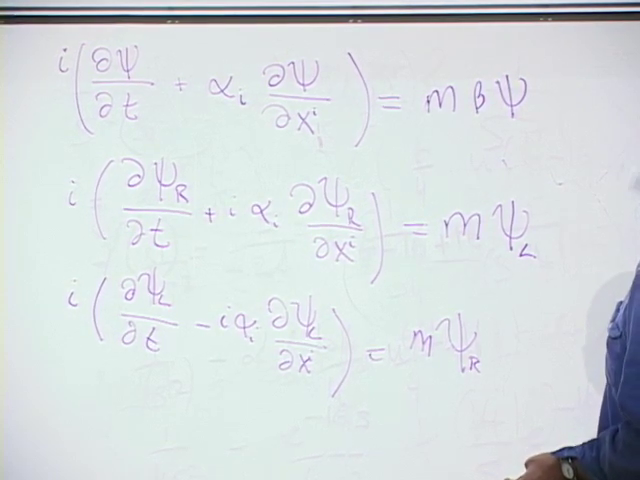
\includegraphics[width=0.74\textwidth]{lecture_09_figure_05.png}
\caption{La pizarra presenta primero la ecuación de Dirac y luego la descompone en ecuaciones acopladas de quiralidad izquierda y derecha.}
\lectureframe{00:40:30}
\label{fig:l09-dirac-board}
\end{figure}

La base quiral hace explícito el papel de \(m\). Con
\(\sigma^\mu=(1,\bm\sigma)\) y
\(\bar\sigma^\mu=(1,-\bm\sigma)\),
\begin{align}
  i\bar\sigma^\mu\partial_\mu\psi_L&=m\psi_R,
  \label{eq:l09-weyl-left}\\
  i\sigma^\mu\partial_\mu\psi_R&=m\psi_L.
  \label{eq:l09-weyl-right}
\end{align}
Cuando \(m=0\), las ecuaciones son independientes: un campo quiral izquierdo y uno quiral derecho pueden propagarse sin interactuar entre sí. Cuando \(m\neq0\), cada uno actúa como fuente del otro. Este es el sentido preciso en que una masa de Dirac mezcla las quiralidades izquierda y derecha.

Susskind describe esto diciendo que el fermión oscila entre los estados de quiralidad izquierda y derecha. Esa forma de expresarlo capta el acoplamiento, pero no debe llevarse hasta una imagen clásica literal de una partícula puntual que alterna de un estado a otro. La afirmación precisa es que la ecuación de campo es acoplada:
\eqref{eq:l09-weyl-left}--\eqref{eq:l09-weyl-right}.

\begin{classroomqa}
\audiencequestion{¿Son coherentes los factores de \(i\) y los signos de las dos ecuaciones de la pizarra?
\lecturetimestamp{00:41:10}}
\lecturerresponse{No, si se comparan línea por línea en la pizarra: durante la derivación rápida se sacó un factor \(i\) de forma inconsistente. Lo fiable es el patrón de acoplamiento. Las ecuaciones \eqref{eq:l09-weyl-left} y
\eqref{eq:l09-weyl-right} corresponden a una convención estándar coherente.}
\end{classroomqa}

\subsection{Por qué la simetría débil prohíbe una masa desnuda}

El término de masa de Dirac correspondiente en el lagrangiano es
\begin{equation}
  \mathcal L_m
  =-m\bar\psi\psi
  =-m\left(\bar\psi_L\psi_R+\bar\psi_R\psi_L\right).
  \label{eq:l09-bare-dirac-mass}
\end{equation}
Bajo la transformación de juguete \eqref{eq:l09-chiral-toy-charge},
\begin{equation}
  \bar\psi_L\psi_R\longmapsto
  e^{-i\theta}\bar\psi_L\psi_R,
  \qquad
  \bar\psi_R\psi_L\longmapsto
  e^{i\theta}\bar\psi_R\psi_L.
\end{equation}
Ninguno de los dos términos es invariante. Por tanto, el coeficiente de mezcla directa entre izquierda y derecha --\(m\) está prohibido antes de la ruptura de simetría.

El electromagnetismo por sí solo no plantearía este problema, porque \(\psi_L\) y \(\psi_R\) tienen la misma carga eléctrica. El obstáculo se debe a que sus números cuánticos débiles son distintos.

\subsection{Preguntas sobre helicidad que ponen de manifiesto la sutileza de la quiralidad}

Ahora la clase pone a prueba desde varios ángulos la imagen intuitiva de la quiralidad. Estas preguntas no son cuestiones secundarias: revelan con precisión dónde resulta útil la helicidad y dónde hay que recurrir a la quiralidad.

\begin{classroomqa}
\audiencequestion{¿Cómo sería el mundo si la interacción débil emitiera electrones de ambas helicidades en igual proporción?
\lecturetimestamp{00:42:12}}
\lecturerresponse{La asimetría de paridad inmediata desaparecería en ese proceso. Pero la teoría electrodébil real es quiral: solo los dobletes de quiralidad izquierda llevan la interacción débil de corriente cargada. La clase pospone una explicación más completa de por qué la naturaleza eligió esa estructura.}
\end{classroomqa}

\begin{classroomqa}
\audiencequestion{Supongamos que se prepara el espín de un electrón en dirección vertical y luego se acelera el electrón horizontalmente. ¿Es levógiro o dextrógiro?
\lecturetimestamp{00:42:44}}
\lecturerresponse{Un estado de espín transversal al momento es una superposición de las dos helicidades. La helicidad está bien definida solo cuando el espín es paralelo o antiparalelo al momento. Aun así, los proyectores quirales débiles del campo están bien definidos.}
\end{classroomqa}

Una partícula masiva puede frenarse hasta quedar en reposo y acelerarse en la dirección opuesta sin invertir su espín. Entonces cambia el signo de su helicidad. Una partícula sin masa no puede ser alcanzada ni llevada al reposo mediante una transformación de Lorentz, así que su helicidad es invariante bajo los boosts propios. Esto motiva la afirmación de la clase de que una especie con una sola helicidad física debe carecer de masa. La formulación más precisa en teoría de campos es que una masa de Dirac invariante de Lorentz requiere ambas quiralidades.

\begin{classroomqa}
\audiencequestion{Un fotón con polarización circular puede reflejarse en un espejo e invertir su dirección sin llegar nunca al reposo. ¿Contradice eso el argumento sobre la helicidad?
\lecturetimestamp{00:45:28}}
\lecturerresponse{No. El espejo es un sistema externo que puede intercambiar momento angular e invertir la dirección de propagación. Un proceso de reflexión no es un boost de Lorentz que alcanza al fotón. La existencia de un canal también depende de los estados de polarización permitidos y de las condiciones de contorno del material.}
\end{classroomqa}

\begin{classroomqa}
\audiencequestion{¿Un haz ordinario de electrones contiene una sola quiralidad o ambas?
\lecturetimestamp{00:46:10}}
\lecturerresponse{En general, ambas. Un estado de electrón masivo contiene componentes de las dos quiralidades, y un haz no polarizado contiene ambas helicidades. Las fuentes especializadas pueden producir un haz polarizado con una marcada asimetría de helicidad.}
\end{classroomqa}

\begin{classroomqa}
\audiencequestion{¿Se puede enfocar un haz sin depender del espín, o los campos magnéticos separan las dos polarizaciones?
\lecturetimestamp{00:46:29}}
\lecturerresponse{El enfoque ordinario de la posición puede ser en gran medida insensible al espín, pero los momentos magnéticos se acoplan a los gradientes del campo magnético. Por tanto, las fuentes selectivas en espín, los gradientes del tipo Stern--Gerlach y la dinámica del espín en los aceleradores permiten preparar o separar polarizaciones.}
\end{classroomqa}

\begin{classroomqa}
\audiencequestion{¿La diferencia entre izquierda y derecha en la interacción débil es simplemente accidental?
\lecturetimestamp{00:48:13}}
\lecturerresponse{En este curso, se considera un hecho experimental incorporado al modelo estándar. Su regularidad hace que no parezca un accidente fortuito, pero el propio modelo estándar no deriva el patrón completo de cargas quirales a partir de un principio más profundo.}
\end{classroomqa}

\section{La construcción de Yukawa}

\subsection{Asignar al Higgs la carga que falta}

La simetría prohíbe una masa numérica, pero permite una interacción con un campo que aporte la fase de transformación que falta. Introduzcamos un escalar complejo tal que
\begin{equation}
  \phi\longmapsto e^{i\theta}\phi,
  \qquad
  \phi^\dagger\longmapsto e^{-i\theta}\phi^\dagger.
  \label{eq:l09-scalar-charge}
\end{equation}
Entonces
\begin{equation}
  \mathcal L_Y
  =-y\,\bar\psi_L\phi\psi_R
   -y^*\,\bar\psi_R\phi^\dagger\psi_L
  \label{eq:l09-yukawa-lagrangian}
\end{equation}
es invariante gauge. En el primer término,
\(\bar\psi_L\) aporta \(e^{-i\theta}\) y \(\phi\) aporta
\(e^{i\theta}\); las fases se cancelan. El segundo término es su conjugado hermítico.

De forma equivalente, las ecuaciones quirales adquieren una mezcla dependiente del campo:
\begin{align}
  i\bar\sigma^\mu D_\mu\psi_L
    &=y\phi\psi_R,
  \label{eq:l09-yukawa-eom-left}\\
  i\sigma^\mu\partial_\mu\psi_R
    &=y^*\phi^\dagger\psi_L.
  \label{eq:l09-yukawa-eom-right}
\end{align}

\begin{figure}[htbp]
\centering
\includegraphics[width=0.76\textwidth]{lecture_09_figure_06.png}
\caption{La masa desnuda de los miembros derechos de las ecuaciones se ha sustituido por el campo escalar cargado. Los signos exactos de la pizarra son esquemáticos; la estructura invariante está dada en \eqref{eq:l09-yukawa-lagrangian}.}
\lectureframe{00:51:30}
\label{fig:l09-yukawa-board}
\end{figure}

Antes de la ruptura de simetría, esto es una interacción, no una masa. Un fermión de quiralidad derecha solo puede convertirse en uno de quiralidad izquierda mientras emite o absorbe el cuanto escalar necesario para equilibrar la carga. El coeficiente \(y\) es un acoplamiento de Yukawa, no la carga gauge \(g\).

\begin{classroomqa}
\audiencequestion{¿Es legítimo simplemente poner \(\phi\) y
\(\phi^\dagger\) en los miembros derechos de las dos ecuaciones?
\lecturetimestamp{00:51:55}}
\lecturerresponse{Es legítimo precisamente porque sus fases de transformación corrigen la discrepancia. La prueba decisiva no es la forma visual de la ecuación, sino la invariancia gauge de la interacción
\(\bar\psi_L\phi\psi_R+\mathrm{h.c.}\).}
\end{classroomqa}

\subsection{El vacío convierte la interacción en masa}

Ahora identifiquemos \(\phi\) con el campo de Higgs y dejemos que alcance un módulo no nulo en el vacío. Con la normalización simplificada de la clase,
\begin{equation}
  \phi\simeq f,
\end{equation}
por lo que \eqref{eq:l09-yukawa-lagrangian} contiene
\begin{equation}
  \mathcal L_Y
  \supset
  -yf\,\bar\psi_L\psi_R
  -y^*f\,\bar\psi_R\psi_L .
\end{equation}
Cuando corresponde, tras una redefinición de fase inocua, la masa del fermión es
\begin{equation}
  m_f=yf.
  \label{eq:l09-lecture-fermion-mass}
\end{equation}
Este es el análogo fermiónico del resultado vectorial \(m_A=gf\). El mismo valor de vacío del Higgs que aporta una polarización longitudinal a los bosones gauge débiles también aporta los números cuánticos débiles que faltan para unir los fermiones de quiralidad izquierda y derecha.

Con la convención de normalización canónica del modelo estándar,
\begin{equation}
  H(x)=\frac1{\sqrt2}
  \begin{pmatrix}
    0\\ v+h(x)
  \end{pmatrix},
  \qquad v\simeq246\ \mathrm{GeV},
  \label{eq:l09-sm-higgs-vacuum}
\end{equation}
y, por tanto,
\begin{equation}
  m_f=\frac{y_fv}{\sqrt2}.
  \label{eq:l09-sm-fermion-mass}
\end{equation}
La cantidad \(f\) de la clase y la cantidad convencional \(v/\sqrt2\) solo difieren por esta elección de normalización.

\begin{classroomqa}
\audiencequestion{Si solo el producto \(yf\) es una masa fermiónica, ¿cómo se pueden determinar por separado el acoplamiento \(y\) y la escala del vacío \(f\)?
\lecturetimestamp{00:55:36}}
\lecturerresponse{Una vez conocidos los acoplamientos gauge, las masas de los bosones gauge débiles determinan la escala del vacío. Después, la masa medida de un fermión determina su acoplamiento de Yukawa. En la teoría completa,
\(m_W=gv/2\), \(m_Z=v\sqrt{g^2+g'^2}/2\) y
\(y_f=\sqrt2m_f/v\).}
\end{classroomqa}

\begin{classroomqa}
\audiencequestion{¿La masa del bosón débil es de unos \(900\ \mathrm{GeV}\)?
\lecturetimestamp{00:57:43}}
\lecturerresponse{No; la clase corrige enseguida el lapsus y da un valor aproximado de \(90\ \mathrm{GeV}\). Más precisamente,
\(m_W\simeq80\ \mathrm{GeV}\) y \(m_Z\simeq91\ \mathrm{GeV}\), mientras que la escala subyacente del vacío es \(v\simeq246\ \mathrm{GeV}\).}
\end{classroomqa}

\subsection{Una sola escala del vacío, muchos acoplamientos de Yukawa}

Cada especie de fermión cargado tiene su propio acoplamiento de Yukawa:
\begin{equation}
  m_i=y_i f
  \qquad\text{(lecture normalization)}.
  \label{eq:l09-mass-family}
\end{equation}

\begin{figure}[htbp]
\centering
\includegraphics[width=0.76\textwidth]{lecture_09_figure_08.png}
\caption{La pizarra resume la dependencia de la especie como \(m_i=g_i f\); los \(g_i\) que aparecen allí son los acoplamientos de Yukawa que aquí llamamos \(y_i\).}
\lectureframe{01:16:30}
\label{fig:l09-mass-family-board}
\end{figure}

Para el electrón, la clase estima
\begin{equation}
  y_e\sim\frac{0.5\ \mathrm{MeV}}{10^2\ \mathrm{GeV}}
  \sim10^{-5}.
\end{equation}
Al usar el valor canónico \(v=246\ \mathrm{GeV}\) se obtiene el valor más preciso
\(y_e\simeq2.9\times10^{-6}\). En el extremo opuesto está el quark top:
\begin{equation}
  y_t=\frac{\sqrt2m_t}{v}\simeq1.
\end{equation}
Así pues, el mecanismo de Higgs explica cómo puede existir una masa invariante gauge, pero no explica la enorme jerarquía entre los \(y_i\). Las masas fermiónicas observadas simplemente traducen esa jerarquía a valores medidos.

\begin{classroomqa}
\audiencequestion{¿De verdad tiene el quark top un acoplamiento de Yukawa de orden unidad?
\lecturetimestamp{00:59:09}}
\lecturerresponse{Sí. Su masa es comparable a la escala electrodébil, así que su acoplamiento no es un número perturbativo diminuto como el del electrón. En la normalización moderna, \(y_t\) es cercano a la unidad.}
\end{classroomqa}

\subsection{Restituir la fluctuación física del Higgs}

Al fijar el escalar en su valor de vacío, ocultamos la excitación radial. Restituyámosla de manera esquemática:
\begin{equation}
  \phi(x)\simeq f+h(x).
\end{equation}
El factor de Yukawa pasa a ser
\begin{equation}
  y\phi\simeq yf+yh=m_f+yh.
  \label{eq:l09-mass-plus-higgs}
\end{equation}

\begin{figure}[htbp]
\centering
\includegraphics[width=0.76\textwidth]{lecture_09_figure_07.png}
\caption{La pizarra restituye la fluctuación del Higgs dentro del término de Yukawa: la parte constante produce la masa fermiónica y la parte fluctuante produce la emisión o absorción de un Higgs.}
\lectureframe{01:01:15}
\label{fig:l09-higgs-fluctuation-board}
\end{figure}

El primer término de \eqref{eq:l09-mass-plus-higgs} es la masa. El segundo es un vértice en el que un bosón de Higgs se acopla al fermión. En la notación canónica del modelo estándar,
\begin{equation}
  \mathcal L_Y
  \supset
  -m_f\bar\psi\psi
  -\frac{m_f}{v}h\bar\psi\psi.
  \label{eq:l09-higgs-fermion-vertex}
\end{equation}
El acoplamiento es proporcional a la masa del fermión. Por tanto, sujeto a las restricciones cinemáticas, los factores de color, el espacio de fases y los canales en competencia, el Higgs se acopla con más intensidad a los fermiones más pesados.

\begin{classroomqa}
\audiencequestion{¿Las constantes de acoplamiento son probabilidades en sí mismas?
\lecturetimestamp{01:03:35}}
\lecturerresponse{Intervienen en las amplitudes cuánticas. A menudo, una tasa sencilla es proporcional al módulo al cuadrado de una amplitud y, por tanto, al cuadrado de un acoplamiento; pero también influyen el espacio de fases, las sumas sobre espín, la interferencia, los lazos y los vértices múltiples. No se debe identificar directamente un acoplamiento con una probabilidad.}
\end{classroomqa}

\begin{classroomqa}
\audiencequestion{¿Este argumento supone que solo hay un campo de Higgs?
\lecturetimestamp{01:03:59}}
\lecturerresponse{Describe el modelo estándar mínimo, que tiene un doblete de Higgs complejo. Tres de sus cuatro componentes reales son absorbidos por \(W^\pm\) y \(Z\), y queda un escalar neutro físico. Las extensiones pueden incluir más dobletes u otros multipletes escalares. Los modelos supersimétricos suelen requerir dos dobletes de Higgs y, por tanto, contienen varios estados físicos del Higgs.}
\end{classroomqa}

Ahora podemos comparar esa expectativa histórica con los experimentos.
\editorialnote{Esta clase se grabó antes del descubrimiento del Higgs. ATLAS y CMS anunciaron en 2012 la observación de una partícula similar al Higgs, cuya masa se mide actualmente en torno a \(125\ \mathrm{GeV}\). Sus acoplamientos observados concuerdan en términos generales con el patrón del modelo estándar, en el que son proporcionales a la masa. La afirmación de que se desintegra preferentemente en partículas más pesadas siempre está sujeta a una salvedad cinemática: un par \(t\bar t\) en la capa de masa no cabe en un Higgs de \(125\ \mathrm{GeV}\).}

\section{Antipartículas, haces y significado de la quiralidad}

Antes de pasar a los neutrinos, la clase retoma varias preguntas prácticas sobre antipartículas y haces de acelerador.

\begin{classroomqa}
\audiencequestion{¿Qué quiralidad tiene la antipartícula de un electrón levógiro?
\lecturetimestamp{01:06:05}}
\lecturerresponse{En el límite ultrarrelativista, un campo electrónico de quiralidad izquierda aniquila electrones de helicidad levógira y crea positrones de helicidad dextrógira. Este es uno de los casos en que hay que distinguir cuidadosamente entre partícula y antipartícula, y entre quiralidad y helicidad.}
\end{classroomqa}

\begin{classroomqa}
\audiencequestion{¿Pueden colisionar un electrón y un positrón para producir un bosón \(Z\)?
\lecturetimestamp{01:07:13}}
\lecturerresponse{Sí, cuando su energía en el centro de masas coincide con la del canal permitido. Los colisionadores de electrones--positrones estudiaron con gran precisión la resonancia del \(Z\). En el proceso completo se conservan la carga y los demás números cuánticos.}
\end{classroomqa}

\begin{classroomqa}
\audiencequestion{¿Se producen todos los positrones mediante un único proceso débil especial?
\lecturetimestamp{01:07:37}}
\lecturerresponse{No. La producción de pares es un proceso electromagnético habitual. Por ejemplo, un electrón energético puede emitir un fotón virtual, que a su vez puede producir un par \(e^-e^+\) en el campo de otra partícula. La clase lo ilustra con un diagrama de Feynman.}
\end{classroomqa}

\begin{classroomqa}
\audiencequestion{¿Puede un acelerador lineal seleccionar la velocidad o la energía de sus electrones?
\lecturetimestamp{01:09:24}}
\lecturerresponse{Sí. Los campos de aceleración y la temporización permiten seleccionar un intervalo de energías. Cuando los electrones ya son ultrarrelativistas, su velocidad está extremadamente cerca de \(c\), así que la energía adicional del acelerador aumenta sobre todo el momento y la energía total, en lugar de aumentar la velocidad de forma apreciable.}
\end{classroomqa}

\begin{classroomqa}
\audiencequestion{¿Puede un acelerador preparar un haz con una sola polarización?
\lecturetimestamp{01:09:47}}
\lecturerresponse{Sí, aunque es técnicamente exigente. Se pueden preparar electrones con espín polarizado a baja energía mediante una fuente que dependa del espín y luego acelerarlos controlando la precesión del espín. Los colisionadores modernos cuantifican la polarización resultante del haz en vez de considerarla perfectamente pura.}
\end{classroomqa}

\section{Masa de los neutrinos y posibilidad de Majorana}

\subsection{Por qué la masa de los neutrinos obligó a ampliar el modelo}

El modelo estándar mínimo original incluía solo campos de neutrino con quiralidad izquierda y, por tanto, predecía neutrinos sin masa. Las oscilaciones de neutrinos muestran que al menos dos de sus autovalores de masa son distintos y que las masas de los neutrinos no son nulas, aunque sean diminutas comparadas con las de los fermiones cargados.

\begin{classroomqa}
\audiencequestion{¿Qué tan pequeñas son las masas de los neutrinos y dónde está su componente de quiralidad derecha?
\lecturetimestamp{01:10:38}}
\lecturerresponse{Las oscilaciones determinan diferencias de masas al cuadrado, no las masas absolutas. Las separaciones pertinentes corresponden a escalas de aproximadamente \(0.009\ \mathrm{eV}\) y \(0.05\ \mathrm{eV}\). Una descripción de Dirac añade neutrinos estériles de quiralidad derecha; una descripción de Majorana, en cambio, relaciona la quiralidad que falta con campos de neutrino conjugados de carga.}
\end{classroomqa}

Para describir un neutrino de Dirac, se añade un nuevo campo \(\nu_R\) y se repite la construcción de Yukawa:
\begin{equation}
  \mathcal L_{\nu,\mathrm{Dirac}}
  =-y_\nu\bar L\,\widetilde H\,\nu_R+\mathrm{h.c.},
  \qquad
  m_\nu=\frac{y_\nu v}{\sqrt2}.
  \label{eq:l09-dirac-neutrino}
\end{equation}
El valor requerido de \(y_\nu\) es extraordinariamente pequeño.

Hay otra posibilidad lógica porque el neutrino no tiene carga eléctrica. Un neutrino de quiralidad izquierda puede acoplarse a su propio conjugado de carga, que tiene la quiralidad opuesta:
\begin{equation}
  \nu_L\longleftrightarrow(\nu_L)^c_R .
  \label{eq:l09-majorana-mixing}
\end{equation}
Un autoestado de masa construido de este modo es un fermión de Majorana: es su propia antipartícula, salvo por convenciones de fase. La mezcla análoga electrón--positrón está prohibida porque violaría la conservación exacta de la carga eléctrica.

\begin{classroomqa}
\audiencequestion{¿Por qué se permite la mezcla partícula--antipartícula para un neutrino, pero no para un electrón?\lecturetimestamp{01:13:43}}
\lecturerresponse{Un electrón y un positrón tienen cargas eléctricas opuestas, así que un término de masa que los mezclara como si fueran el mismo estado de una partícula violaría la simetría electromagnética no rota. Un neutrino es eléctricamente neutro. Si ningún número leptónico exactamente conservado lo distingue de su antipartícula, se permite una masa de Majorana.}\end{classroomqa}

El nombre honra a Ettore Majorana, el joven físico italiano que formuló este tipo de representación de fermión real y desapareció en 1938. La conferencia se detiene en el misterio histórico: nunca se llegó a esclarecer qué fue de él.
\editorialnote{Antes de la ruptura electrodébil, una masa de Majorana invariante gauge para el neutrino activo del modelo estándar no puede aparecer como término desnudo renormalizable. A bajas energías puede surgir del operador de Weinberg de dimensión cinco
\((LH)(LH)/\Lambda\), o mediante un mecanismo seesaw que involucre neutrinos estériles pesados. Aún no se ha determinado experimentalmente si los neutrinos son partículas de Dirac o de Majorana.}

\section{Por qué el espectro familiar se agrupa cerca de la escala electrodébil}

\subsection{La escala común y sus importantes salvedades}

\begin{classroomqa}
\audiencequestion{¿Por qué se esperaba que la masa del Higgs estuviera al alcance de la escala débil?\lecturetimestamp{01:14:48}}
\lecturerresponse{La curvatura del potencial de Higgs determina la masa radial del Higgs, mientras que la misma escala del vacío \(f\) determina las masas de \(W\) y \(Z\). Por tanto, si el acoplamiento propio del escalar no era extremo, se esperaba que la masa del Higgs fuera, en términos generales, del orden de la escala débil. El valor observado de \(125\ \mathrm{GeV}\) se encuentra efectivamente en ese rango.}
\end{classroomqa}

El resumen más llamativo de la conferencia es que las masas elementales del modelo estándar mínimo se remontan a un único vacío roto:
\begin{align}
  m_W&=\frac12gv,\\
  m_Z&=\frac12\sqrt{g^2+g'^2}\,v,\\
  m_f&=\frac1{\sqrt2}y_fv.
  \label{eq:l09-electroweak-mass-summary}
\end{align}
Si \(v\) se anulara manteniendo fijos los acoplamientos adimensionales, los bosones gauge débiles y los fermiones elementales cargados no tendrían masa.

Esta afirmación no debe extenderse más allá de su ámbito. El fotón y los gluones siguen sin masa porque una simetría gauge no rota los protege. La mayor parte de la masa del protón y del neutrón es energía de enlace de la QCD, no la suma de las masas de sus quarks debidas al Higgs. La masa de los neutrinos requiere una extensión del modelo mínimo. La masa del propio Higgs depende del potencial escalar y no es simplemente otra masa de Yukawa.

\subsection{Partículas cuya masa no tiene por qué esperar a la ruptura de simetría}

Supongamos que un fermión nuevo tuviera componentes de quiralidad izquierda y derecha con números cuánticos gauge idénticos. Entonces,
\(\bar\Psi_L\Psi_R+\mathrm{h.c.}\) ya sería invariante gauge. Un fermión \emph{vectorial} así podría tener una masa desnuda \(M\), independiente de
\(v\):
\begin{equation}
  \mathcal L_{\mathrm{vectorlike}}
  =-M\bar\Psi\Psi.
  \label{eq:l09-vectorlike-mass}
\end{equation}
No hay ningún impedimento de simetría electrodébil para que \(M\gg v\).

Esto motiva el argumento general de naturalidad de la conferencia. Las partículas protegidas por una simetría gauge o quiral siguen sin masa hasta que el vacío del Higgs rompe esa protección, así que sus masas están ligadas a la escala relativamente pequeña \(v\). Las partículas que carecen de tal protección pueden tener de forma natural masas mucho mayores y, por tanto, estar ausentes del espectro observado a bajas energías. Lo que vemos podría ser un efecto de selección: las partículas accesibles son aquellas cuyas masas estaban obligadas a esperar a la ruptura electrodébil.

\begin{classroomqa}
\audiencequestion{¿Las partículas con masas independientes mucho mayores no tendrían ningún papel en la realidad?\lecturetimestamp{01:19:39}}
\lecturerresponse{Tendrían poca importancia en la física de laboratorio ordinaria a bajas energías, porque son difíciles de producir, pero aun así podrían influir en la historia de altas energías o en la cosmología. La conferencia menciona la materia oscura como un posible ámbito en el que un espectro oculto más pesado podría manifestarse por primera vez.}
\end{classroomqa}

La discusión de 2010 refleja la expectativa, popular entonces, de que la materia oscura tuviera una masa de escala débil o algo mayor. Esa sigue siendo una clase útil de modelos, pero no es un hecho establecido. La materia oscura se ha detectado gravitacionalmente, pero se desconocen tanto su identidad como partícula como el origen de su masa.

\section{Preguntas finales: rayos cósmicos, inercia, gravedad y quiralidad}

\subsection{La masa no es energía alta en el laboratorio}

\begin{classroomqa}
\audiencequestion{¿Cuál es la masa de un rayo cósmico?
\lecturetimestamp{01:20:57}}
\lecturerresponse{Un rayo cósmico puede ser un protón, un núcleo atómico, un electrón o un fotón; su masa invariante es la masa de esa partícula o sistema. Lo espectacular es su energía en el laboratorio, que en los eventos de mayor energía alcanza aproximadamente desde \(10^{20}\) hasta \(10^{21}\ \mathrm{eV}\). Una energía alta no es lo mismo que una masa invariante alta.}
\end{classroomqa}

Un rayo cósmico choca contra una partícula blanco que está aproximadamente en reposo. Para un protón proyectil de energía de laboratorio \(E\gg m_p\),
\begin{equation}
  s=(p_1+p_2)^2
  \simeq2m_pE+2m_p^2,
  \qquad
  \sqrt{s}\simeq\sqrt{2m_pE}.
  \label{eq:l09-fixed-target-s}
\end{equation}
Solo la raíz cuadrada de la energía del proyectil se convierte en energía del centro de masas. Para haces iguales que chocan frontalmente, cada uno con energía \(E_{\rm beam}\),
\begin{equation}
  \sqrt{s}\simeq2E_{\rm beam}.
  \label{eq:l09-collider-s}
\end{equation}
Por eso, un colisionador es mucho más eficiente que un blanco fijo para convertir la energía controlada de los haces en masa de nuevas partículas.

\begin{classroomqa}
\audiencequestion{¿Por qué el colisionador del CERN puede ser una sonda más potente que una sola partícula, mucho más energética, que golpea materia en reposo?
\lecturetimestamp{01:21:50}}
\lecturerresponse{En una colisión con blanco fijo, la conservación del momento hace que la mayor parte de la energía de laboratorio siga adelante en el movimiento del estado final. En un colisionador simétrico, el momento espacial total puede anularse, de modo que la energía de los haces queda disponible como energía del centro de masas. Los rayos cósmicos de mayor energía pueden superar al LHC en \(\sqrt{s}\), pero llegan de manera impredecible y no pueden proporcionar ni la luminosidad de un colisionador ni un entorno controlado para los detectores.}
\end{classroomqa}

\subsection{Masa en reposo y resistencia a la aceleración}

\begin{classroomqa}
\audiencequestion{¿Son, en esencia, lo mismo la inercia y la masa?
\lecturetimestamp{01:22:41}}
\lecturerresponse{En reposo, la masa invariante es tanto la energía en reposo, mediante \(E_0=mc^2\), como el parámetro que determina la respuesta a una fuerza a bajas velocidades. La relatividad especial explica por qué ambas definiciones corresponden a una misma magnitud. Para cuerpos en movimiento, es más claro mantener fija la masa invariante y describir la aceleración mediante la energía y el momento relativistas.}
\end{classroomqa}

La relación invariante
\begin{equation}
  E^2=p^2c^2+m^2c^4
  \label{eq:l09-energy-momentum}
\end{equation}
contiene ambos significados. Cerca del reposo,
\begin{equation}
  E=mc^2+\frac{p^2}{2m}+\cdots,
\end{equation}
por lo que la misma \(m\) que da la energía en reposo aparece en la respuesta cinética. A altas velocidades, la relación entre fuerza y aceleración depende de si la fuerza es paralela o perpendicular a la velocidad. Esta dependencia direccional explica por qué los tratamientos modernos evitan una \emph{masa relativista} dependiente de la velocidad y reservan el término masa para la magnitud invariante de Lorentz \(m\).

\subsection{A qué se acopla la gravedad}

\begin{classroomqa}
\audiencequestion{Cuando el Higgs confiere masa a una partícula, ¿empieza entonces a acoplarse a la gravedad?\lecturetimestamp{01:23:58}}
\lecturerresponse{Su energía en reposo contribuye a la gravedad, pero la masa no es la única fuente. Los fotones no tienen masa y, aun así, la gravedad los desvía. En relatividad general, la fuente es el tensor de energía--momento: la densidad de energía, el flujo de momento, la presión y los esfuerzos. Para la materia que se mueve lentamente, la contribución dominante es su energía de masa en reposo.}
\end{classroomqa}

La desviación de la luz cerca del Sol ilustra este punto de manera directa. Un fotón responde a la curvatura del espacio-tiempo pese a que \(m=0\), y su energía y momento también contribuyen al campo gravitatorio. Para dos cuerpos masivos casi estáticos, la energía está dominada por \(mc^2\), así que la gravedad newtoniana puede expresarse en términos de sus masas sin presentar la formulación más general del tensor de energía--momento.

\begin{classroomqa}
\audiencequestion{¿Cuesta más acelerar una partícula de alta energía de la misma manera en todas las direcciones?\lecturetimestamp{01:25:20}}
\lecturerresponse{No. El cambio de momento producido por una fuerza paralela al movimiento difiere del que produce una fuerza transversal. Es cierto que cuesta más desviar una partícula de mayor energía, pero asignarle una única masa aumentada por estar en movimiento oculta esta estructura direccional.}
\end{classroomqa}

\subsection{Un electrón en reposo y la distinción prometida}

\begin{classroomqa}
\audiencequestion{¿Cómo puede decirse que un electrón en reposo tiene helicidad izquierda o derecha?\lecturetimestamp{01:26:32}}
\lecturerresponse{No se le puede asignar helicidad en reposo, porque la helicidad depende de la dirección del momento. Aun así, un espinor en reposo puede descomponerse en componentes de quiralidad izquierda y derecha. En un electrón con masa están presentes ambas componentes, y el término de masa las acopla.}
\end{classroomqa}

\begin{classroomqa}
\audiencequestion{Si un electrón en reposo no tiene helicidad, ¿puede aun así participar en una interacción débil?\lecturetimestamp{01:27:18}}
\lecturerresponse{Sí. La interacción débil se acopla a la quiralidad, no a una etiqueta de helicidad que depende del sistema de referencia. A altas energías, la helicidad es una aproximación práctica a la quiralidad; cerca del reposo, esa simplificación deja de funcionar. Esta es la sutil distinción que la conferencia había dejado pendiente.}
\end{classroomqa}

\section{Preguntas históricas del final de la conferencia}

\subsection{La ventana del Higgs antes de su descubrimiento}

En 2010 todavía no se había observado el Higgs. Los observables electrodébiles de precisión, en especial las relaciones sensibles a los efectos de lazos entre \(W\), \(Z\), el quark top y otros parámetros, favorecían un Higgs relativamente ligero dentro del modelo estándar. La conferencia cita una región superior probable cercana a \(160\ \mathrm{GeV}\), muy por debajo de \(v\), aunque sin una diferencia de un orden de magnitud.

\begin{classroomqa}
\audiencequestion{¿Qué indicios sugerían entonces que el Higgs era más ligero que la escala del vacío \(250\ \mathrm{GeV}\)\lecturetimestamp{01:28:28}}?
\lecturerresponse{Las mediciones de alta precisión podían compararse con correcciones radiativas cuyos valores dependen logarítmicamente de la masa del Higgs. Los ajustes globales resultantes favorecían un Higgs ligero. Era evidencia indirecta, no una medición directa de la masa; el valor directo medido posteriormente es de aproximadamente \(125\ \mathrm{GeV}\).}
\end{classroomqa}

\begin{classroomqa}
\audiencequestion{¿Podrían varios mínimos del potencial de Higgs producir distintos valores de \(f\), quizá vinculados a diferentes generaciones de partículas?
\lecturetimestamp{01:29:28}}
\lecturerresponse{Distintos mínimos pueden dar lugar a una física muy diferente a bajas energías, pero no se puede deducir fácilmente que haya varios mínimos del Higgs a partir de las generaciones observadas. La conferencia aplaza el tema más amplio de los múltiples vacíos para un curso posterior, en vez de dar aquí la impresión de resolverlo.}
\end{classroomqa}

\begin{classroomqa}
\audiencequestion{¿Se esperaba que el Higgs fuera la primera partícula nueva descubierta en el LHC?\lecturetimestamp{01:31:32}}
\lecturerresponse{No necesariamente. Su visibilidad depende de las tasas de producción y de los canales de desintegración, algunos de los cuales pueden ser difíciles de detectar o invisibles. Antes de los datos del LHC, era plausible que aparecieran primero partículas supersimétricas u otras partículas nuevas. Históricamente, se descubrió el Higgs y todavía no se ha confirmado ninguna partícula supersimétrica.}
\end{classroomqa}

\subsection{Cuándo una partícula neutra es su propia antipartícula}

\begin{classroomqa}
\audiencequestion{¿Carecen el fotón y el gluón de antipartículas porque no tienen masa?\lecturetimestamp{01:32:12}}
\lecturerresponse{No. La ausencia de masa no es el criterio. El fotón es su propia antipartícula porque ninguna carga conservada distingue un fotón de un antifotón. Cada gluón también es un cuanto gauge autoconjugado en la representación de color correspondiente, aunque los propios gluones llevan color y sus etiquetas de color se mezclan bajo conjugación de carga. El neutrón es eléctricamente neutro, pero tiene un antineutrón distinto porque el número bariónico y su contenido de quarks los distinguen.}
\end{classroomqa}

El neutrino vuelve a ser el caso sutil. Tiene interacciones débiles, y los estados ultrarrelativistas llamados neutrino y antineutrino interactúan con helicidades opuestas. Si un número leptónico exacto los distingue, pueden formar una partícula de Dirac con una antipartícula distinta. Si el número leptónico no es exacto y la masa es de Majorana, la partícula masiva es su propia antipartícula, aunque sus dos estados de helicidad se comporten de manera diferente en los procesos débiles.

\begin{classroomqa}
\audiencequestion{¿La carga débil y el número leptónico demuestran que los neutrinos y los antineutrinos tienen que ser distintos?\lecturetimestamp{01:32:46}}
\lecturerresponse{No de manera concluyente. Las interacciones débiles distinguen los estados de helicidad, pero una masa de Majorana puede combinar un campo de neutrino con su conjugado de carga. La cuestión decisiva es si existe un número cuántico conservado exactamente que prohíba esa mezcla. El modelo estándar no impone el número leptónico total como una simetría gauge exacta.}
\end{classroomqa}

Las oscilaciones ordinarias de sabor requieren una salvedad aparte.
\editorialnote{Las oscilaciones de sabor observadas habitualmente mezclan los estados \(\nu_e,\nu_\mu,\nu_\tau\) del mismo sector de neutrinos o de antineutrinos; por sí solas no demuestran la conversión de neutrinos--antineutrinos. Los procesos que violan el número leptónico, como la desintegración doble beta sin neutrinos, aportarían evidencia directa de una masa de Majorana, pero todavía no se ha confirmado ninguno.}

\begin{classroomqa}
\audiencequestion{¿Explica el modelo estándar por qué están cuantizadas las cargas eléctricas?\lecturetimestamp{01:33:39}}
\lecturerresponse{La conferencia reconoce la pregunta, pero no la desarrolla. Dentro del modelo estándar, la invariancia gauge y la cancelación de anomalías restringen fuertemente las asignaciones coherentes de hipercarga; una explicación más profunda suele recurrir a la gran unificación o a otras estructuras ultravioletas.}
\end{classroomqa}

\section{Lo que ha establecido la conferencia}

Ahora encajan las explicaciones de los bosones gauge y los fermiones.

\begin{enumerate}\item Una teoría gauge que solo contiene términos con derivadas no tiene brecha de energía para un potencial vectorial homogéneo. La simetría gauge prohíbe una masa vectorial desnuda.
  \item Un escalar cargado con magnitud de vacío no nula aporta \(g^2f^2A_\mu A^\mu\). Su modo de Goldstone angular se convierte en la polarización longitudinal de un bosón gauge débil masivo.
  \item Una masa de Dirac acopla \(\psi_L\) y \(\psi_R\). Como la interacción débil les asigna números cuánticos gauge distintos, está prohibido un término de masa desnudo que mezcle las componentes de quiralidad izquierda--derecha.
  \item Una interacción de Yukawa inserta el campo de Higgs entre las dos quiralidades y es invariante gauge. Al sustituir el Higgs por su valor de vacío se obtiene \(m_f=y_ff\), mientras que al conservar su fluctuación se obtiene el acoplamiento físico Higgs--fermión.
  \item La masa del neutrino sigue la misma lógica de quiralidad izquierda--derecha, pero admite realizaciones tanto de Dirac como de Majorana porque el neutrino es eléctricamente neutro.
  \item Las partículas que no tienen protección gauge o quiral podrían tener masas independientes de la escala electrodébil y situarse muy por encima de los experimentos actuales.
\end{enumerate}

La afirmación unificadora, por tanto, no es que el Higgs sea una sustancia que arrastre mecánicamente a las partículas. Es que el vacío electrodébil tiene un parámetro de orden escalar no nulo. Ese parámetro de orden cambia qué términos invariantes gauge son posibles en las ecuaciones de baja energía. En el caso de los vectores, abre una brecha a momento cero; en el de los fermiones, permite la mezcla de quiralidades izquierda--derecha. Así, las distintas masas miden acoplamientos distintos al mismo vacío roto.
